\section{課題 3 演習ガイド}
%
%%% RECENT CRYPTGRAPY
%
\subsection{現代の暗号方式}
\begin{frame}[containsverbatim,shrink]
\frametitle{現代の暗号方式}
\framesubtitle{Optional}
  \begin{itemize}
\item シーザ暗号では暗号化と復号に同じ鍵をもちいていました
\item 暗号化と復号で異なる鍵を使用する暗号について紹介します
    \begin{itemize}
\item 公開鍵暗号方式 (Public Key Crpptography)
    \end{itemize}
  \end{itemize}
\end{frame}
\begin{frame}[containsverbatim,shrink]
\frametitle{公開鍵暗号方式}
  \begin{itemize}
\item Bob さんは Alice さんに自身の公開鍵を送る
\item Bob さんにメッセージを送るときは Alice さんは Bob さんの公開鍵で暗号化する
\item Alice さんはメッセージを受け取ったら,自身の秘密鍵で復号する
\item 逆に,Alice さんが送るときは Alice さんの秘密鍵で暗号化し, Bob さんは Alice さんの公開鍵で復号する
  \end{itemize}
  \begin{center}
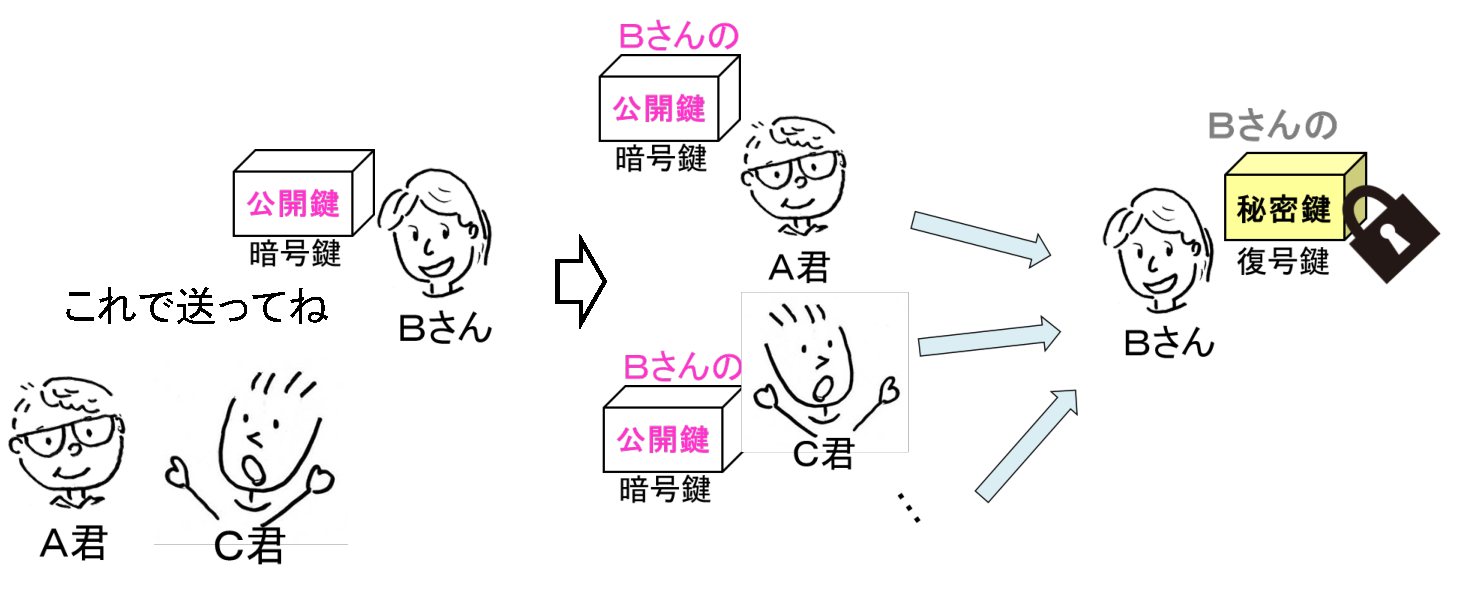
\includegraphics[scale=0.5]{./Figure/elementaryCS-figPublicKey.pdf}
  \end{center}
\end{frame}
\begin{frame}[containsverbatim,shrink]
\frametitle{公開鍵暗号方式 (Public Key Cryptography)}
  \begin{itemize}
\item Diffie-Hellman 方式
\item RSA
  \end{itemize}
  \begin{block}{Public key cryptosystem の特徴}
    \begin{enumerate}
\item 適当な鍵が与えられているときはメッセージを暗号化,復号することが容易
\item 公開鍵から秘密鍵を予測することは困難\label{num:infeasible}
    \end{enumerate}
  \end{block}
\end{frame}
\begin{frame}[shrink]
\frametitle{Diffie-Hellman Key Exchange}
  \begin{block}{原理}
    \begin{itemize}
\item \(b^k=g \mod p\) の $k$ を求める問題に置き換えられる
    \end{itemize}
  \end{block}
  \begin{enumerate}
\item 大きな素数 $p$ と $g$ の組をひとつ選ぶ (\href{https://www.ietf.org/rfc/rfc3526.txt}{\beamerbutton{RFC 3526}})
    \begin{itemize}
\item \(p=17, g=3\)
    \end{itemize}
\item Alice と Bob はそれぞれ秘密鍵をえらぶ
    \begin{itemize}
\item \(k_{private}^{Alice}=15, k_{private}^{Bob}=13\)
    \end{itemize}
\item 公開鍵をそれぞれ計算して交換する\label{num:publickey}
    \begin{itemize}
\item \(k_{public}^{Alice}=g^{k_{private}^{Alice}}\mod 17=3^{15}\mod 17=6\)
\item \(k_{public}^{Bob}=g^{k_{private}^{Bob}}\mod 17=3^{13}\mod 17=12\)
    \end{itemize}
\item Bob は Alice の公開鍵で共有秘密鍵を計算する
    \begin{itemize}
\item \(S_{Bob,Alice}=(k_{public}^{Alice})^{k_{private}^{Bob}}\mod p=6^{13}\mod 17=10\)
    \end{itemize}
\item Alice は Bob の公開鍵で共有秘密鍵を計算する
    \begin{itemize}
\item \(S_{Alice,Bob}=(k_{public}^{Bob})^{k_{private}^{Alice}}\mod p=12^{15}\mod 17=10\)
    \end{itemize}
  \end{enumerate}
\end{frame}
\subsection{課題 3 のシチュエーション}
\begin{frame}[containsverbatim,label=situation,shrink]
\frametitle{課題 3 のシチュエーション}
  \begin{itemize}
\item Alice と Bob が通信しているとして,そこに Eve (eavesdropper) がいるとします
\item 通信の内容を盗み見られないように暗号化して通信します
\item 暗号化の手順は以下の通り
    \begin{enumerate}
\item 送りたい文 (平文 $m$) を暗号化 (encryption) して暗号文 $c$ を作成
\item 暗号文 $c$ を送信
\item 暗号文 $c$ を受信
\item 暗号文 $c$ を復号 (decryption) して平文 $m$ を得る
    \end{enumerate}
\item Eve はこの通信の内容を盗み見ようと試みる (暗号解読を試みる)
  \end{itemize}
  \begin{center}
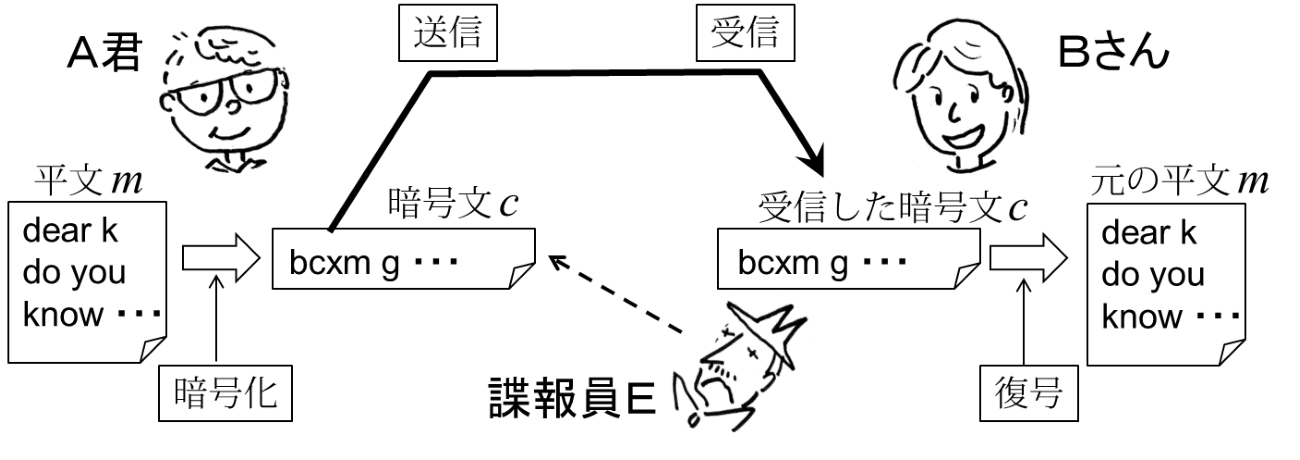
\includegraphics[scale=0.3]{./Figure/elementaryCS-figAliceBob.pdf}
  \end{center}
\hfill{\hyperlink{function}{\beamerbutton{Back to function-slide}}}
\end{frame}
\subsection{課題 3 テーマ}
\begin{frame}[containsverbatim,shrink]
\frametitle{課題 3 ガイド}
  \begin{block}{課題 3 テーマ}
暗号解読に挑戦
  \end{block}
  \begin{itemize}
\item 課題 3 で作成してほしいプログラム
    \begin{itemize}
\item 暗号解読プログラム: kaidoku.py
\item オプション:
      \begin{itemize}
\item 講義で説明していない暗号方式 myango.py, myhukogo.py と
\item その暗号を解読するための自分流のプログラム mykaidoku.py
      \end{itemize}
    \end{itemize}
  \end{itemize}
\end{frame}
\begin{frame}[containsverbatim,shrink]
\frametitle{作業内容}
  \begin{itemize}
\item code.py での文字列操作を参考に ango.py, hukugo.py を完成させてみてください
\item それが終わったら kaidoku.py を作ってみてください
\item リダイレクトやパイプを使う
  \end{itemize}
  \begin{itembox}{暗号化するとき}
 python3 ango.py < plaintext.txt
  \end{itembox}
  \begin{itembox}{復号するとき}
 python3 hukugou.py < chiphertext.txt
  \end{itembox}
  \begin{itembox}{暗号化して復号するとき}
 python3 ango.py < plaintext.txt | python3 hukugo.py
  \end{itembox}
\end{frame}
\begin{frame}[containsverbatim,shrink]
\frametitle{リダイレクションとパイプ}
  \begin{itemize}
\item OS には標準入力や標準出力という概念があります
\item 通常は標準入力はキーボード,標準出力はディスプレイを指しています
\item プログラムが入力を読み取る場合,特に指定がなければ標準入力から読み込み,
\item 出力する場合は標準出力に書き込みます
\item リダイレクションは標準入出力をファイルに変更します
\item パイプ | はプログラムの出力を別のプログラムの入力につなげる役割します
\item >! とびっくりをつけると上書きします
  \end{itemize}
  \begin{itembox}{入力リダイレクション}
 python3 ango.py < plaintext.txt
  \end{itembox}
  \begin{itembox}{出力リダイレクション}
 python3 ango.py > chiphertext.txt
  \end{itembox}
  \begin{itembox}{パイプ}
 python3 ango.py | python3 hukugo.py
  \end{itembox}
\end{frame}
\begin{frame}[containsverbatim,shrink]
\frametitle{暗号解読のヒント}
  \begin{itemize}
\item 意味をなす一般的な文章では文字の出現頻度には偏りがあります
\item たとえば英語では母音 e が最も出現頻度が高い
\item シーザ暗号はこの出現頻度は暗号化しても偏りは変わりません
\item この特徴を利用して何文字移動しているかを予測することができます
\item 各文字 26 個の頻度を計算するために出現回数を要素とする配列をつくる
  \end{itemize}
  \begin{center}
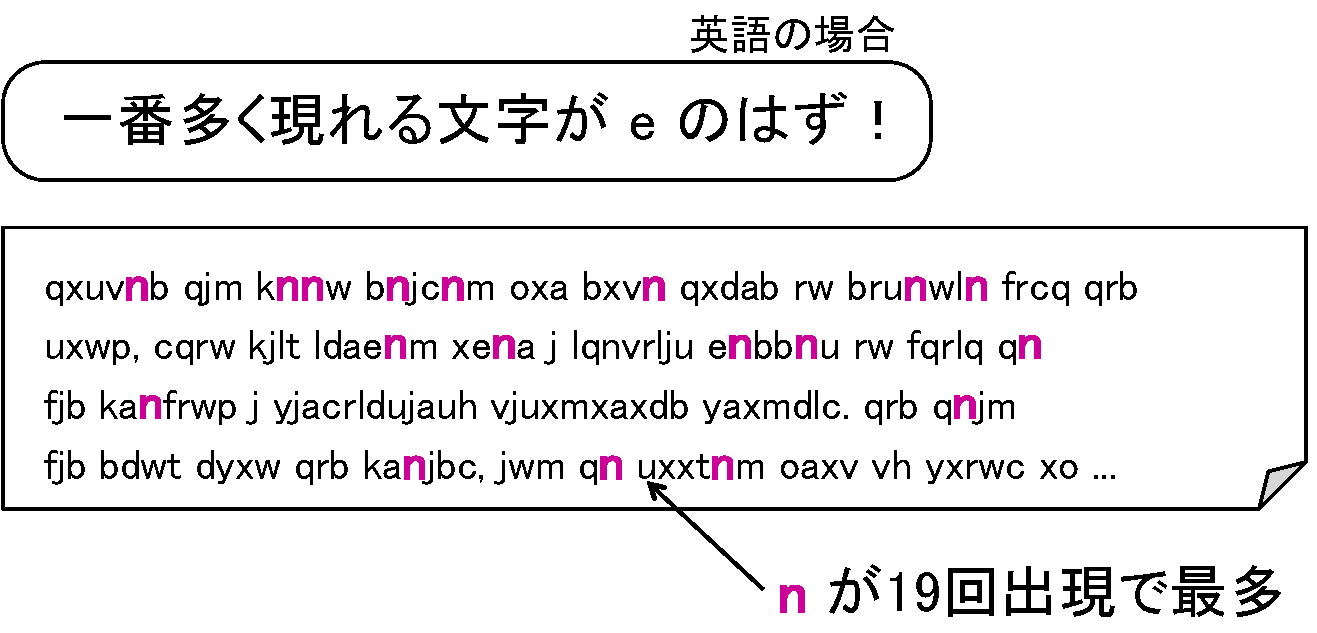
\includegraphics[scale=0.3]{./Figure/elementaryCS-figHintForCryptoanalysis.pdf}
  \end{center}
\end{frame}
\begin{frame}[containsverbatim,shrink]
\frametitle{暗号解読のヒント\textemdash つづき}
  \begin{itemize}
\item 13 番目の文字 n が最多なので 4 番目の文字 e にシフト
\item \(13-4=9\) なので 9 文字シフトしていると推測できる
  \end{itemize}
  \begin{center}
\includegraphics[scale=0.3]{./Figure/elementaryCS-figHindo.pdf}
  \end{center}
\end{frame}
\begin{frame}[containsverbatim,shrink]
\frametitle{暗号解読のヒント\textemdash より高度な方法}
  \begin{itemize}
\item フォーマルには各文字の出現頻度と暗号文での出現頻度の相関\(\phi(i)\)をとります
\item \(\phi(i)=\Sigma_{0\leq c\leq 25}f(c)p(c-i)\), ここで \(f(c)=\frac{n_c}{l_{ct}}\) は暗号文での文字 c の出現頻度,\(p(c-i)\) は一般の出現頻度とする
\item \href{https://sites.google.com/a/presystems.xyz/sample/home/elementary-computer-science}{\beamerbutton{https://sites.google.com/a/presystems.xyz/sample/home/elementary-computer-science}}に置いてある 1-gram.txt が出現頻度のファイルです
\item 相関係数 \(\phi(i)\) が
    \begin{itemize}
\item $1$ に近いほど: \(f(c)\) が大きくなれば \(p(c-i)\) も大きくなり相関が強くなる
\item $0$ 近傍: \(f(c)\) と \(p(c-i)\) はあまり相関がない
    \end{itemize}
  \end{itemize}
\end{frame}
%\begin{frame}[fragile]
%\frametitle{仮引数と実引数}
%\scriptsize
%  \begin{itemize}
%\item 関数は仮引数というものをもつ
%    \begin{itemize}
%\scriptsize
%\item 下の例では {\tt guess, x} が仮引数
%    \end{itemize}
%\item 複数の関数が同じ名前の仮引数を持っていても良い
%\item 仮引数は関数の本体で有効である
%\item 関数を呼び出したときの値に束縛 (bind) されて,関数の本体では呼び出し時の値に置き換えられる
%\item 呼び出し時の値を実引数という
%\item 一般に変数は有効範囲 (scope) が決まっている
%\item 仮引数は関数本体が有効範囲である
%  \end{itemize}
%  \begin{columns}[c]
%    \begin{column}{0.5\textwidth}
%      \begin{lstlisting}[caption={Newton 法},label=newton-rec]
%### Newton's method 
%def sqrt_iter (guess,x)
%  if is_enough(guess,x) then
%     return(guess)
%  else
%     return(sqrt_iter(improve(guess,x),x))
%  end
%end
%      \end{lstlisting}
%    \end{column}
%    \begin{column}{0.45\textwidth}
%      \begin{lstlisting}[caption={Newton 法},label=newton-is_enough-rec]
%def is_enough (guess,x)
%  return(abs((square(guess)-x))<0.001)
%end
%      \end{lstlisting}
%    \end{column}
%  \end{columns}
%\end{frame}
